\subsection*{Syfte}
%För att illustrera hur en atom endast absorberar specifika nivåer av energi kan man accelerera elektroner genom ett moln av atomer, i detta fall Kvicksilver (Hg). 
%Detta experiment kallas ``Frank-Hertz experiment'' och är det första experimentet att tydligt visa atomers kvantnivåer.

Frank-Hertz experiment är ett av de första experimenten uppbyggda med avsikten att studera kvantisering av energin i valenselektroner, utfört av James Frank och Gustav Hertz 1914.  Experimentet utförs här i avsikt att fördjupa förståelse för kvantisering av energi, och var den resulterande kvantmekaniken avviker från klassisk mekanik.

\subsection*{Teori}
%En elektrons energi kan bestämmas av dess kinetiska energi. För att kunna exitera en Kvicksilveratom måste denna energi stämma perfekt överrens med exitationsenergin för ett av atomens elektronlager.
%Denna lab undersöker vid vilka spänningar vi har toppar och bottnar för att avgöra energin. Denna energi kan beräknas till en våglängd av ljus och på så sätt jämföras mot dess ljusspektra, se \autoref{fig:hgspec}.% och \autoref{fig:hgwl}.

Grundstommen som experimentet baseras på är vakumrörteknologi; en apparat som i modern tid näst intill ersatts av transistorn i de flesta användsningsområdena på grund av dess begränsningar som gjort den inkompatibel med modern höghastighetselektronik.

Det klassiska vakumröret består av katoden, ett upphettat filament som avger sig elektroner till sin omgivning; anoden, en fysiskt separat ledare mot vilken de frigjorda elektronerna attraheras med hjälp av en pålagd spänning; samt gallret, ett nät placerat mellan anoden och katoden och vars spänning kontrolleras relativt de andra två för att modulera strömmen som färdas emellan dom.

Principen som experimentet baseras på är att vakumröret i detta fall innehåller kvicksilver som kommer förångas vid upphettningen av kammaren röret placerats i. När kammaren och katoden är upphettade kommer en spänning läggas mellan katoden och anoden vilket kommer driva elektroner därimellan som ger upphov till en mätbar ström. Med hjälp av en transresistiv\footnote{Omvandlar en strömsignal till en spänningsignal} förstärkare och ett oscilloskop så kan strömmen grafas mot den pålagda spänningen. 

Under experimentet kommer även gallret att backspännas. Detta kommer motverka elektronerna som propagerar mot anoden genom att introducera ett potentialsteg som kan styras. Detta tillåter en arbiträr barriär för att kunna attenuera elektronflödet utöver drivspänningen och elektrånernas interaktion med kvicksilvret. 

\begin{figure}[h]
	\centering
	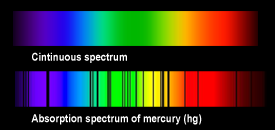
\includegraphics[width=.7\textwidth]{HgSpec.png}
	\caption{Kvicksilver absorbtionsspectrum.\cite{astronoo}}
	\label{fig:hgspec}
\end{figure}

%\begin{figure}[h]
%	\centering
%	\begin{subfigure}[c]{0.63\textwidth}
%	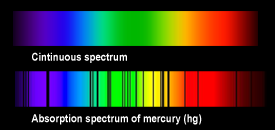
\includegraphics[width=\textwidth]{HgSpec.png}
%	\caption{Kvicksilver absorbtionsspectrum.\cite{astronoo}}
%	\label{fig:hgspec}
%	\end{subfigure}
%	~
%	\begin{subfigure}[c]{0.32\textwidth}
%	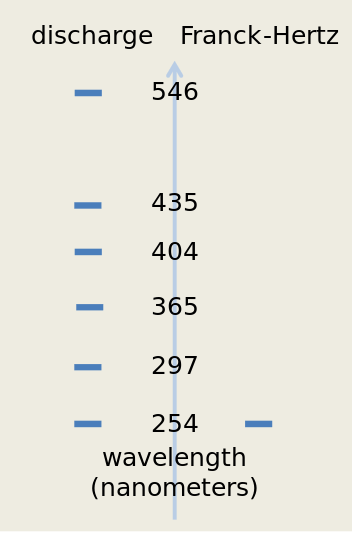
\includegraphics[width=\textwidth]{HgWavelen.png}
%	\caption{Take this picture away.}
%	\label{fig:hgwl}
%	\end{subfigure}
%	\caption{stuff}\label{fig:hgstuff}
%\end{figure}
